\documentclass[tikz,border=4pt]{standalone}
\usepackage{ctex}
\usepackage{amsmath}
\usepackage{pgfplots}
\pgfplotsset{compat=1.18}

% p10-06e: 图象法解不等式——开口向上，y>0的x范围在两侧，y<0在中间
% y = x^2-4x+3，零点x=1和x=3
\begin{document}
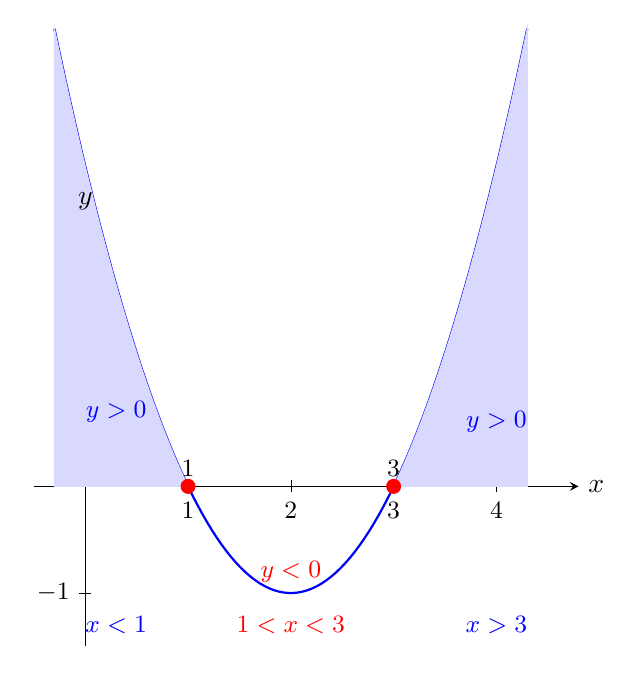
\begin{tikzpicture}
\begin{axis}[
  width=8.5cm, height=7cm,
  axis lines=center,
  xlabel={$x$}, ylabel={$y$},
  every axis x label/.style={at={(axis cs:4.8,0)}, anchor=west},
  every axis y label/.style={at={(axis cs:0,2.5)}, anchor=south},
  xmin=-0.5, xmax=4.8,
  ymin=-1.5, ymax=2.5,
  xtick={1,2,3,4},
  ytick={-1,1,2},
  tick style={color=black},
  ticklabel style={font=\small},
  clip=false,
]
  % y = x^2 - 4x + 3
  \addplot[blue, thick, domain=-0.3:4.3, samples=100] {x^2 - 4*x + 3};

  % y>0 的区间（两侧着色）
  \addplot[blue!15, fill=blue!15, domain=-0.3:1, samples=30] {max(x^2-4*x+3, 0)} \closedcycle;
  \addplot[blue!15, fill=blue!15, domain=3:4.3, samples=30] {max(x^2-4*x+3, 0)} \closedcycle;

  % 零点
  \addplot[only marks, mark=*, mark size=2.5pt, red] coordinates {(1,0) (3,0)};
  \node[above] at (axis cs:1,0) {\small$1$};
  \node[above] at (axis cs:3,0) {\small$3$};

  % 标注区域
  \node[blue, font=\small] at (axis cs:0.3, 0.7) {$y>0$};
  \node[blue, font=\small] at (axis cs:4.0, 0.6) {$y>0$};
  \node[red, font=\small] at (axis cs:2.0, -0.8) {$y<0$};

  % 解集标注
  \node[font=\small, blue] at (axis cs:0.3, -1.3) {$x<1$};
  \node[font=\small, blue] at (axis cs:4.0, -1.3) {$x>3$};
  \node[font=\small, red] at (axis cs:2.0, -1.3) {$1<x<3$};
\end{axis}
\end{tikzpicture}
\end{document}
